\documentclass[11pt,a4paper]{article}

\usepackage[utf8]{inputenc}
\usepackage[T1]{fontenc}
\usepackage{geometry}

\usepackage{amsmath, amssymb, amsfonts, amsthm, mathtools, bm, mathrsfs, dsfont}
\usepackage{graphicx}
\usepackage{booktabs}
\usepackage{multirow}
\usepackage{longtable}
\usepackage{array}
\usepackage{float}
\usepackage{enumitem}
\usepackage{xcolor}
\usepackage{caption}
\usepackage{algorithm}
\usepackage{algpseudocode}
\usepackage[skins,breakable]{tcolorbox}
\usepackage{fancyhdr}
\usepackage{titlesec}
\usepackage{listings}
\usepackage{tikz}
\usepackage{pgfplots}
\usepackage{hyperref}
\usepackage{microtype}
\usepackage{scalerel}
\usepackage{natbib}
\usepackage{doi}
\usetikzlibrary{arrows.meta,positioning,shapes.geometric,calc}
\pgfplotsset{compat=1.17}

% ========== GEOMETRY ==========
\geometry{left=2.5cm, right=2.5cm, top=3cm, bottom=3cm, headheight=15pt}

% ========== COLOR PALETTE ==========
\definecolor{mistyblue}{HTML}{A3BFD9}
\definecolor{slateblue}{HTML}{7A90B2}
\definecolor{sagegreen}{HTML}{A3BFA3}
\definecolor{dustyteal}{HTML}{6E8B8B}
\definecolor{softgray}{HTML}{D8D8D8}
\definecolor{deepmutedblue}{HTML}{4A5A6A}
\definecolor{signcol}{RGB}{210, 115, 115}      % Soft red
\definecolor{expcol}{RGB}{95, 170, 110}       % Soft green
\definecolor{mantcol}{RGB}{95, 150, 200}      % Soft blue
\definecolor{int8col}{RGB}{160, 125, 185}     % Soft purple
\definecolor{int4col}{RGB}{215, 140, 90}      % Soft orange
% ========== HYPERREF ==========
\hypersetup{
  colorlinks=true,
  linkcolor=deepmutedblue,
  citecolor=slateblue,
  urlcolor=dustyteal,
  pdftitle={Mathematical and Algorithmic Foundations of Deep Neural Networks},
  pdfauthor={Your Name}
}

% ========== TITLE FORMATTING ==========
\titleformat{\section}{\Large\bfseries\color{deepmutedblue}}{\thesection}{1em}{}
[\vspace{-0.5em}\textcolor{mistyblue}{\rule{\textwidth}{2pt}}]
\titleformat{\subsection}{\large\bfseries\color{slateblue}}{\thesubsection}{1em}{}
\titleformat{\subsubsection}{\normalsize\bfseries\color{dustyteal}}{\thesubsubsection}{1em}{}

% =========================
% Paragraph / Subparagraph styling
% =========================
% Place this after your \titleformat declarations in the preamble.

% Paragraph: bold, slightly larger, colored, with a thin dividing rule
\titleformat{\paragraph}[block]
{\normalfont\normalsize\bfseries\color{mantcol}} % formatting of the title
{}                                             % no label (unnumbered)
{0pt}                                          % separation between label and title
{ }                                            % before-code
[\vspace{0.6ex}\color{mistyblue}\rule{\linewidth}{0.8pt}\vspace{0.6ex}] % after-code: thin rule

\titlespacing*{\paragraph}{0pt}{1.0\baselineskip}{0.6\baselineskip}
%           ^left ^before-space ^after-space

% Subparagraph: smaller, italic, muted color, with a faint rule
\titleformat{\subparagraph}[block]
{\normalfont\normalsize\itshape\color{int4col}} % formatting of the title
{}                                             % no label (unnumbered)
{0pt}                                          % separation
{ }                                            % before-code
[\vspace{0.4ex}\color{softgray}\rule{0.95\linewidth}{0.5pt}\vspace{0.4ex}] % after-code: faint rule

\titlespacing*{\subparagraph}{0pt}{0.7\baselineskip}{0.4\baselineskip}

\newcommand{\mainp}[1]{%
  \par\medskip
  {\noindent\bfseries\normalsize\color{mantcol}#1\par}%
  \vspace{0.4ex}%
  {\noindent\color{mistyblue}\rule{\linewidth}{0.8pt}\par}%
  \vspace{0.8ex}%
}

\newcommand{\problemp}[1]{%
  \par\medskip
  {\noindent\bfseries\normalsize\color{signcol}#1\par}%
  \vspace{0.4ex}%
  {\noindent\color{softgray}\rule{\linewidth}{0.6pt}\par}%
  \vspace{0.8ex}%
}

% ========== HEADER AND FOOTER ==========
\pagestyle{fancy}
\fancyhf{}
\fancyhead[L]{\color{dustyteal}\small Quantization}
\fancyhead[R]{\color{dustyteal}\small\thepage}
\renewcommand{\headrulewidth}{0.5pt}
\renewcommand{\headrule}{\hbox to\headwidth{\color{softgray}\leaders\hrule height \headrulewidth\hfill}}

\theoremstyle{definition}
\newtheorem{definition}{Definition}[section]
\newtheorem{theorem}{Theorem}[section]
\newtheorem{lemma}{Lemma}[section]
\newtheorem{corollary}{Corollary}[section]
\newtheorem{proposition}{Proposition}[section]

\tcolorboxenvironment{theorem}{
  colback=mistyblue!20,
  colframe=slateblue,
  fonttitle=\bfseries,
  coltitle=deepmutedblue,
  breakable,
  before skip=1em,
  after skip=1em
}
\tcolorboxenvironment{definition}{
  colback=sagegreen!20,
  colframe=dustyteal,
  fonttitle=\bfseries,
  coltitle=deepmutedblue,
  breakable,
  before skip=1em,
  after skip=1em
}

\newtcolorbox{calloutbox}[2][]{
  colback=sagegreen!15,
  colframe=sagegreen,
  arc=3mm,
  boxrule=1pt,
  left=10pt,
  right=10pt,
  top=10pt,
  bottom=10pt,
  fonttitle=\bfseries\color{deepmutedblue},
  title=#2,
  #1,
  breakable
}
\newtcolorbox{abstractbox}{
  colback=mistyblue!15,
  colframe=mistyblue,
  arc=0mm,
  boxrule=0pt,
  leftrule=4pt,
  rightrule=0pt,
  toprule=0pt,
  bottomrule=0pt,
  left=15pt,
  right=10pt,
  top=10pt,
  bottom=10pt,
  breakable
}
\newtcolorbox{remark}{
  colback=dustyteal!15,
  colframe=dustyteal,
  arc=0mm,
  boxrule=0pt,
  leftrule=4pt,
  rightrule=0pt,
  toprule=0pt,
  bottomrule=0pt,
  left=15pt,
  right=10pt,
  top=10pt,
  bottom=10pt,
  breakable
}
\newtcolorbox{mathasidebox}[2][]{
  colback=softgray!30,
  colframe=slateblue,
  fonttitle=\bfseries,
  coltitle=deepmutedblue,
  title=#2,
  #1,
  breakable
}

\geometry{
  margin=1in,
  headheight=14pt
}

\title{\textbf{ Quantization Techniques for Transformer based Natural Language Processing Models}}

\begin{document}

\maketitle


\section{Related Work}

\subsection{Post-Training Quantization:}
Post training quantization refers to a process that reduces numerical precision in neural network parameters and activations after full training of such model. It reduces model size, decreases memory demand, and may increase execution speed while keeping accuracy close to the original. This approach avoids retraining and offers a direct path from a heavy model to a compact one without structural change but may require dequantization during inference.

Through the research we can distinguish four types of post-training quantization: rotation based, saliency based, optimization based, and compensation based. Each type carries its own properties. A detailed discussion of these methods follows in the next section.

\begin{figure}[h!]
  \centering
  \makebox[\textwidth][c]{%
    
\includegraphics[scale=0.25]{4canvas.png}%
  }
  \caption{Four types of post-training quantization: rotation based, saliency based, optimization based, and compensation based.}
  \label{fig:type_of_ptq}
\end{figure}

\subsubsection{Rotation-Based}
This class relies on structured transformations that soften outliers before quantization, often with the need to sudy the behavior of weights and activation matrices to deduce their distribution.
The central idea is to reshape the weight space through orthogonal operations so the distribution becomes more uniform and less prone to large deviations.

\mainp{QuaRot}

\begin{figure}[h!]
  \hspace*{1cm}
  \makebox[\textwidth][c]{%
    
\includegraphics[scale=0.4]{canv44as.png}%
  }
  \caption{QuaRot applied to a LLaMa-style FFN. RMSNorm scaling ($\alpha$) is absorbed into the weights. Hidden state $X$ is rotated by $Q$, canceled by $Q^\top$ in the first two weights. Weights and activations are INT4; matmul yields INT32, cast and scaled to FP16. While in FP16, a Hadamard transform is applied before quantizing and computing a modified down-proj, producing rotated output $YQ$.}
  \label{fig:quarot}
\end{figure}

\problemp{Problem Statement}
While quantization reduces these costs, quantizing \textit{activations} to low bit-widths (e.g., 4-bit) is difficult due to the presence of large outlier features (channels with consistently high magnitudes). Previous works rely on mixed-precision inference or complex calibration to handle these outliers, which introduces computational overhead and prevents true end-to-end 4-bit integer arithmetic.

\vspace{1cm}
\problemp{Methodology}
QuaRot introduces a quantization scheme based on rotations that eliminates outliers from the hidden states, making weights, activations, and the KV cache amenable to 4-bit quantization without performance degradation. The method operates in two main phases:

\subparagraph{Phase 1: Rotations via Computational Invariance}
The core principle is \textit{Computational Invariance}, which states that the weights and activations in a transformer can be transformed by an orthogonal matrix $\bm{Q}$ without affecting the model output. This relies on the commutation property with RMSNorm:
\begin{equation}
  \text{RMSNorm}(\bm{X}) = \text{RMSNorm}(\bm{X}\bm{Q}^\top)\bm{Q}
\end{equation}
QuaRot fuses randomized Hadamard transformations into the model weights to rotate the activation space, smoothing out outliers.

\begin{itemize}
  \item \textbf{Stage 1a: Weight Modification (Global Rotation).}
    The scaling parameters $\bm{\alpha}$ of RMSNorm are absorbed into adjacent weight matrices. A randomized Hadamard matrix $\bm{Q}$ is applied to rotate the hidden state $\bm{X}$. For a weight matrix $\bm{W}_{in}$ (e.g., $\bm{W}_k, \bm{W}_q$), the modification is:
    \begin{equation}
      \bm{W}_{in} \leftarrow \bm{Q}^\top \text{diag}(\bm{\alpha}) \bm{W}_{in}
    \end{equation}
    Consequently, the activations between blocks become $\bm{X} \leftarrow \bm{X}\bm{Q}$.

  \item \textbf{Stage 1b: FFN Activation Rotation.}
    To remove outliers within the Feed-Forward Network (FFN), a Hadamard transformation $\bm{H}$ is inserted on-the-fly. This operation is fused into the down-projection weight $\bm{W}_{\text{down}}$:
    \begin{equation}
      \bm{W}_{\text{down}} \leftarrow \bm{H} \bm{W}_{\text{down}}}
    \end{equation}

  \item \textbf{Stage 1c \& 1d: Attention and KV Cache.}
    Outliers exist in Keys ($\bm{K}$) and Values ($\bm{V}$). QuaRot applies Hadamard transformations to the attention heads. For the value projection $\bm{W}_v$ and output projection $\bm{W}_{\text{out}}$, with head dimension $d_h$:
    \begin{equation}
      \bm{W}_v \leftarrow \bm{W}_v (\bm{I} \otimes \bm{H}_{d_h}), \quad \bm{W}_{\text{out}} \leftarrow (\bm{I} \otimes \bm{H}_{d_h}) \bm{W}_{\text{out}}
    \end{equation}
    Similar rotations are applied to Queries ($\bm{Q}$) and Keys ($\bm{K}$), allowing the KV cache to be stored in 4-bit precision.
\end{itemize}

\subparagraph{Phase 2: Quantization}
With the signal rotated and outliers removed ("incoherence processing"), the model is quantized:
\begin{itemize}
  \item \textbf{Weights:} Quantized using GPTQ (or RTN) to 4 bits.
  \item \textbf{Activations:} Quantized on-the-fly using symmetric per-token quantization.
  \item \textbf{KV Cache:} Quantized using asymmetric group-wise quantization.
\end{itemize}

\problemp{Key Properties and Results}
\begin{itemize}
  \item \textbf{End-to-End 4-bit:} It is the first method to quantize weights, activations, and KV cache to 4 bits (A4W4KV4) simultaneously.
  \item \textbf{Outlier Elimination:} The rotation leads to an "outlier-free" distribution, significantly reducing quantization error for activations.
  \item \textbf{Performance:} Achieves up to $3.33\times$ speedup in the prefill stage and $3.89\times$ memory savings during decoding on Llama-2-70B compared to FP16.
  \item \textbf{Accuracy:} The 4-bit Llama-2-70B model retains 99\% of zero-shot performance with negligible perplexity degradation (0.47 loss on WikiText-2).
  \item \textbf{Lossless at Higher Bits:} Provides lossless 6-bit and 8-bit models using simple Round-to-Nearest (RTN) quantization without calibration data.
\end{itemize}



\mainp{QuIP}

\begin{figure}[h!]
  \hspace*{0cm}
  \makebox[\textwidth][c]{%
    
\includegraphics[scale=0.23]{quip_methodology (3).png}%
  }
  \caption{QuIP Methodology. The approach tackles the "proxy gap" in 2-bit quantization. It transforms the Hessian and Weights into an incoherent basis using Kronecker-factored orthogonal matrices ($U$ and $V$). It then employs LDLQ, a coordinate-descent algorithm using the $LDL^T$ decomposition of the inverse Hessian, to quantize weights while correcting errors in the remaining full-precision weights.}
  \label{fig:quip_architecture}
\end{figure}

\problemp{Problem Statement}
Existing PTQ methods (e.g., GPTQ) minimize a layer-wise quadratic proxy loss $\mathcal{L}(\hat{\bm{W}}) = (\bm{W}-\hat{\bm{W}})^\top \bm{H} (\bm{W}-\hat{\bm{W}})$. At 4-bits, this proxy correlates well with the actual task loss. However, at \textbf{2-bits}, this correlation breaks down (the "Proxy Gap").
The Hessian $\bm{H}$ for LLMs is highly "coherent" ,dominated by a few large eigenvalues (outlier features). In this regime, standard greedy quantization (rounding to nearest) yields worst-case errors $O(N)$ because the error vectors align with the large eigenvalues of $\bm{H}$.

\vspace{1cm}
\problemp{Methodology}
QuIP provides the first theoretical analysis of 2-bit quantization, proving that quantization error can be bounded by controlling the incoherence of the weight and Hessian matrices. The method consists of three tightly coupled components:

\subparagraph{1. The Proxy Objective and Incoherence}
The method minimizes the quadratic proxy. The theoretical key is that if $\bm{W}$ and $\bm{H}$ are $\mu$-incoherent, the quantization error behaves like random noise rather than worst-case adversarial noise.
QuIP applies an orthogonal transform to "whiten" the problem. Given input $\bm{X}$ and weights $\bm{W}$:
\begin{equation}
  \min_{\hat{\bm{W}}} \|\bm{W}\bm{X} - \hat{\bm{W}}\bm{X}\|_2^2 \implies \min_{\hat{\bm{W}}} \text{Tr}((\tilde{\bm{W}} - \hat{\tilde{\bm{W}}})^\top \tilde{\bm{H}} (\tilde{\bm{W}} - \hat{\tilde{\bm{W}}}))
\end{equation}
The weights and Hessian are transformed via random orthogonal matrices $\bm{U}$ and $\bm{V}$:
\begin{equation}
  \tilde{\bm{W}} = \bm{U}\bm{W}\bm{V}^\top, \quad \tilde{\bm{H}} = \bm{V}\bm{H}\bm{V}^\top
\end{equation}
Here, $\bm{V}$ spreads the singular values of the Hessian (making $\tilde{\bm{H}}$ well-conditioned/incoherent), and $\bm{U}$ ensures the weights themselves are incoherent (flat magnitude distribution). $\bm{U}, \bm{V}$ are constructed using Kronecker products of Hadamard matrices to ensure multiplication in $O(d \log d)$ time.

\subparagraph{2. LDLQ Algorithm (LDL-based Quantization)}
QuIP introduces \textbf{LDLQ}, an iterative coordinate-descent algorithm. Unlike standard rounding, LDLQ utilizes the Cholesky decomposition of the inverse Hessian to update unquantized weights optimally.
Let $\bm{H}^{-1} = \bm{L}\bm{D}\bm{L}^\top$. The quantization error for the $j$-th weight affects the remaining weights via the dependency structure in $\bm{L}$. The algorithm iterates $j = 1 \dots d$:
\begin{itemize}
  \item \textbf{Residual Update:} Calculate the residual error induced by quantizing previous columns.
  \item \textbf{Quantization:} Quantize the current element $\tilde{w}_{j}$ based on the diagonal entry $\bm{D}_{jj}$ and the accumulated error.
  \item \textbf{Error Propagation:} The quantization error $\delta_j$ is propagated to future columns $k > j$ using the non-zero off-diagonals of $\bm{L}$:
    \begin{equation}
      \tilde{w}_k \leftarrow \tilde{w}_k - \frac{\bm{L}_{kj}}{\bm{L}_{jj}} \delta_j
    \end{equation}
\end{itemize}
This is equivalent to Optimal Brain Surgeon (OBS) but implemented efficiently via the fixed $\bm{L}$ from the inverse Hessian decomposition.

\subparagraph{3. Theoretical Bound (The Guarantee)}
QuIP proves that for a block size $n$, if the Hessian and weights are sufficiently incoherent (via the transformations in Step 1), the proxy square loss decreases at a rate of:
\begin{equation}
  \text{Loss} \le O\left(\frac{1}{n}\right) \cdot \mathbb{E}[\text{RoundOffError}]
\end{equation}
This bound guarantees that with large enough block sizes and proper incoherence processing, the 2-bit quantization error will not diverge, effectively "smoothing" the optimization landscape.

\problemp{Key Properties and Results}
\begin{itemize}
  \item \textbf{LDLQ vs GPTQ:} While GPTQ uses Cholesky on $\bm{H}$, LDLQ uses Cholesky on $\bm{H}^{-1}$ (conceptually equivalent via block inversion formulas) but combined with the incoherence transform, LDLQ prevents the "outlier" columns from destroying the quantization of subsequent columns.
  \item \textbf{Scalability via Kronecker:} The use of Kronecker-structured Hadamard matrices allows the transforms to be applied to LLaMa-70B scale models without exploding memory or compute ($O(N^2)$ vs $O(N^3)$).
  \item \textbf{Large Block Sizes:} QuIP demonstrates that larger quantization block sizes reduce the theoretical error bound, a property not exploited by previous per-channel methods.
  \item \textbf{State-of-the-art 2-bit:} QuIP was the first method to generate non-random output for LLaMa-2-70B at 2-bit precision, significantly outperforming OPTQ and GPTQ, which collapse at this bit-width.
\end{itemize}

\mainp{DuQuant}

\begin{figure}[h!]
  \hspace*{1cm}
  \makebox[\textwidth][c]{%
    
\includegraphics[scale=0.53]{duquant_architecture.png}%
  }
  \caption{Overview of the DuQuant Dual Transformation methodology. Unlike pure rotation methods (QuaRot) that only mix channels, DuQuant identifies "Massive Outliers" that survive rotation. It applies a Dual Transformation $\bm{T} = \bm{R} \cdot \bm{S}$ composed of an orthogonal Rotation ($\bm{R}$) to flatten the distribution and a learned Smoothing scaling ($\bm{S}$) to balance the quantization difficulty between Weights and Activations. This is applied omni-directionally to FFNs, Attention, and the KV Cache.}
  \label{fig:duquant}
\end{figure}

\problemp{Problem Statement}
While rotation-based methods (like QuaRot) successfully mitigate "normal" outliers by spreading them across channels, they fail to handle \textbf{Massive Outliers} inherent in newer architectures like Llama-3 and StarCoder2.
Specifically, in the inputs to the FFN down-projection and Attention output projection, outliers with magnitudes up to $1000\times$ the median persist even after Hadamard rotations. These massive outliers dominate the quantization range, leading to substantial accuracy degradation in 4-bit weight-activation (W4A4) settings. Pure rotation is insufficient because it distributes the outlier's energy but does not reduce the aggregate quantization difficulty.

\vspace{1cm}
\problemp{Methodology}
DuQuant proposes a \textbf{Dual Transformation} strategy that mathematically fuses Rotation and Smoothing into a single unified transform $\bm{T}$. This minimizes the quantization error by balancing the "outlier burden" between weights and activations.

\subparagraph{Phase 1: The Dual Transformation ($\bm{T}$)}
The core innovation is combining channel mixing (Rotation) with channel scaling (Smoothing). For an activation $\bm{X}$ and weight $\bm{W}$, the system aims to find a transformation $\bm{T}$ such that the quantized counterparts $\hat{\bm{X}}$ and $\hat{\bm{W}}$ minimize the reconstruction error. The transformation is defined as:
\begin{equation}
  \bm{T} = \bm{R} \cdot \bm{S}
\end{equation}
where $\bm{R}$ is an orthogonal rotation matrix and $\bm{S}$ is a diagonal smoothing matrix.
\begin{itemize}
  \item \textbf{Rotation ($\bm{R}$):} Uses Randomized Hadamard Transformations (RHT) to mix channels, reducing the \textit{number} of outlier channels by delocalizing features.
  \item \textbf{Smoothing ($\bm{S}$):} Addresses the \textit{magnitude} of the remaining massive outliers. By scaling down the activation channels with high variance and scaling up the corresponding weight channels, $\bm{S}$ migrates the quantization difficulty from $\bm{X}$ to $\bm{W}$, which has higher capacity (or is easier to quantize).
\end{itemize}

\subparagraph{Phase 2: Optimization of Scales}
Unlike SmoothQuant, which uses heuristic scales, DuQuant derives the optimal smoothing scales $\bm{S} = \text{diag}(\bm{s})$ by minimizing the combined quantization error of weights and activations. The objective function is formulated as:
\begin{equation}
  \min_{\bm{s}} \left( \|\bm{X}\text{diag}(\bm{s})^{-1} - Q(\bm{X}\text{diag}(\bm{s})^{-1})\|_F^2 + \lambda \|\text{diag}(\bm{s})\bm{W} - Q(\text{diag}(\bm{s})\bm{W})\|_F^2 \right)
\end{equation}
This convex optimization ensures that the "Massive Outliers" in activations are suppressed ($\bm{s}_i > 1$) just enough so that the resulting increased magnitude in the weights $\bm{W}$ does not degrade weight quantization performance.

\subparagraph{Phase 3: Omni-directional Implementation}
DuQuant applies this dual transformation to all linear layers and the KV Cache:
\begin{itemize}
  \item \textbf{FFN & Attention:} The transform $\bm{T}$ is absorbed into the weights. For a layer $\bm{Y} = \bm{X}\bm{W}$, the operation becomes:
    \begin{equation}
      \bm{Y} = (\bm{X}\bm{T}^{-1}) (\bm{T}\bm{W}) \approx Q_{\text{A}}(\bm{X}\bm{T}^{-1}) \cdot Q_{\text{W}}(\bm{T}\bm{W})
    \end{equation}
  \item \textbf{KV Cache:} The Key and Value matrices are also subjected to the Dual Transformation, enabling low-bit (4-bit) KV caching without the precision loss seen in standard rotational methods.
\end{itemize}

\problemp{Key Properties and Results}
\begin{itemize}
  \item \textbf{Massive Outlier Suppression:} DuQuant effectively reduces the kurtosis of activation distributions in Llama-3-70B, converting spiky "massive" outliers into a Gaussian-like distribution amenable to uniform quantization.
  \item \textbf{Llama-3 Capability:} It is one of the first methods to successfully quantize Llama-3-70B to W4A4 with negligible performance loss (retaining 98\%+ of FP16 accuracy), a model where QuaRot typically fails due to extreme outlier magnitudes.
  \item \textbf{Better than Rotation Alone:} Ablation studies show that $\bm{R} \cdot \bm{S}$ (Dual) consistently outperforms $\bm{R}$ (QuaRot/QuIP) and $\bm{S}$ (SmoothQuant) individually, proving that "mixing" and "scaling" are complementary necessities for low-bit LLMs.
  \item \textbf{Hardware Efficient:} The smoothing scales and rotations are fused offline. During inference, the computational graph remains identical to a standard quantized transformer (Int4 MatMul), incurring no runtime overhead.
\end{itemize}

\subsubsection{Salience-Based}
This class assigns precision according to weight importance.
The guiding principle is to preserve high-impact weights with higher precision and quantize low-impact ones to lower bitwidths.

\mainp{AWQ}

\begin{figure}[h!]
  \hspace*{0cm}
  \makebox[\textwidth][c]{%
    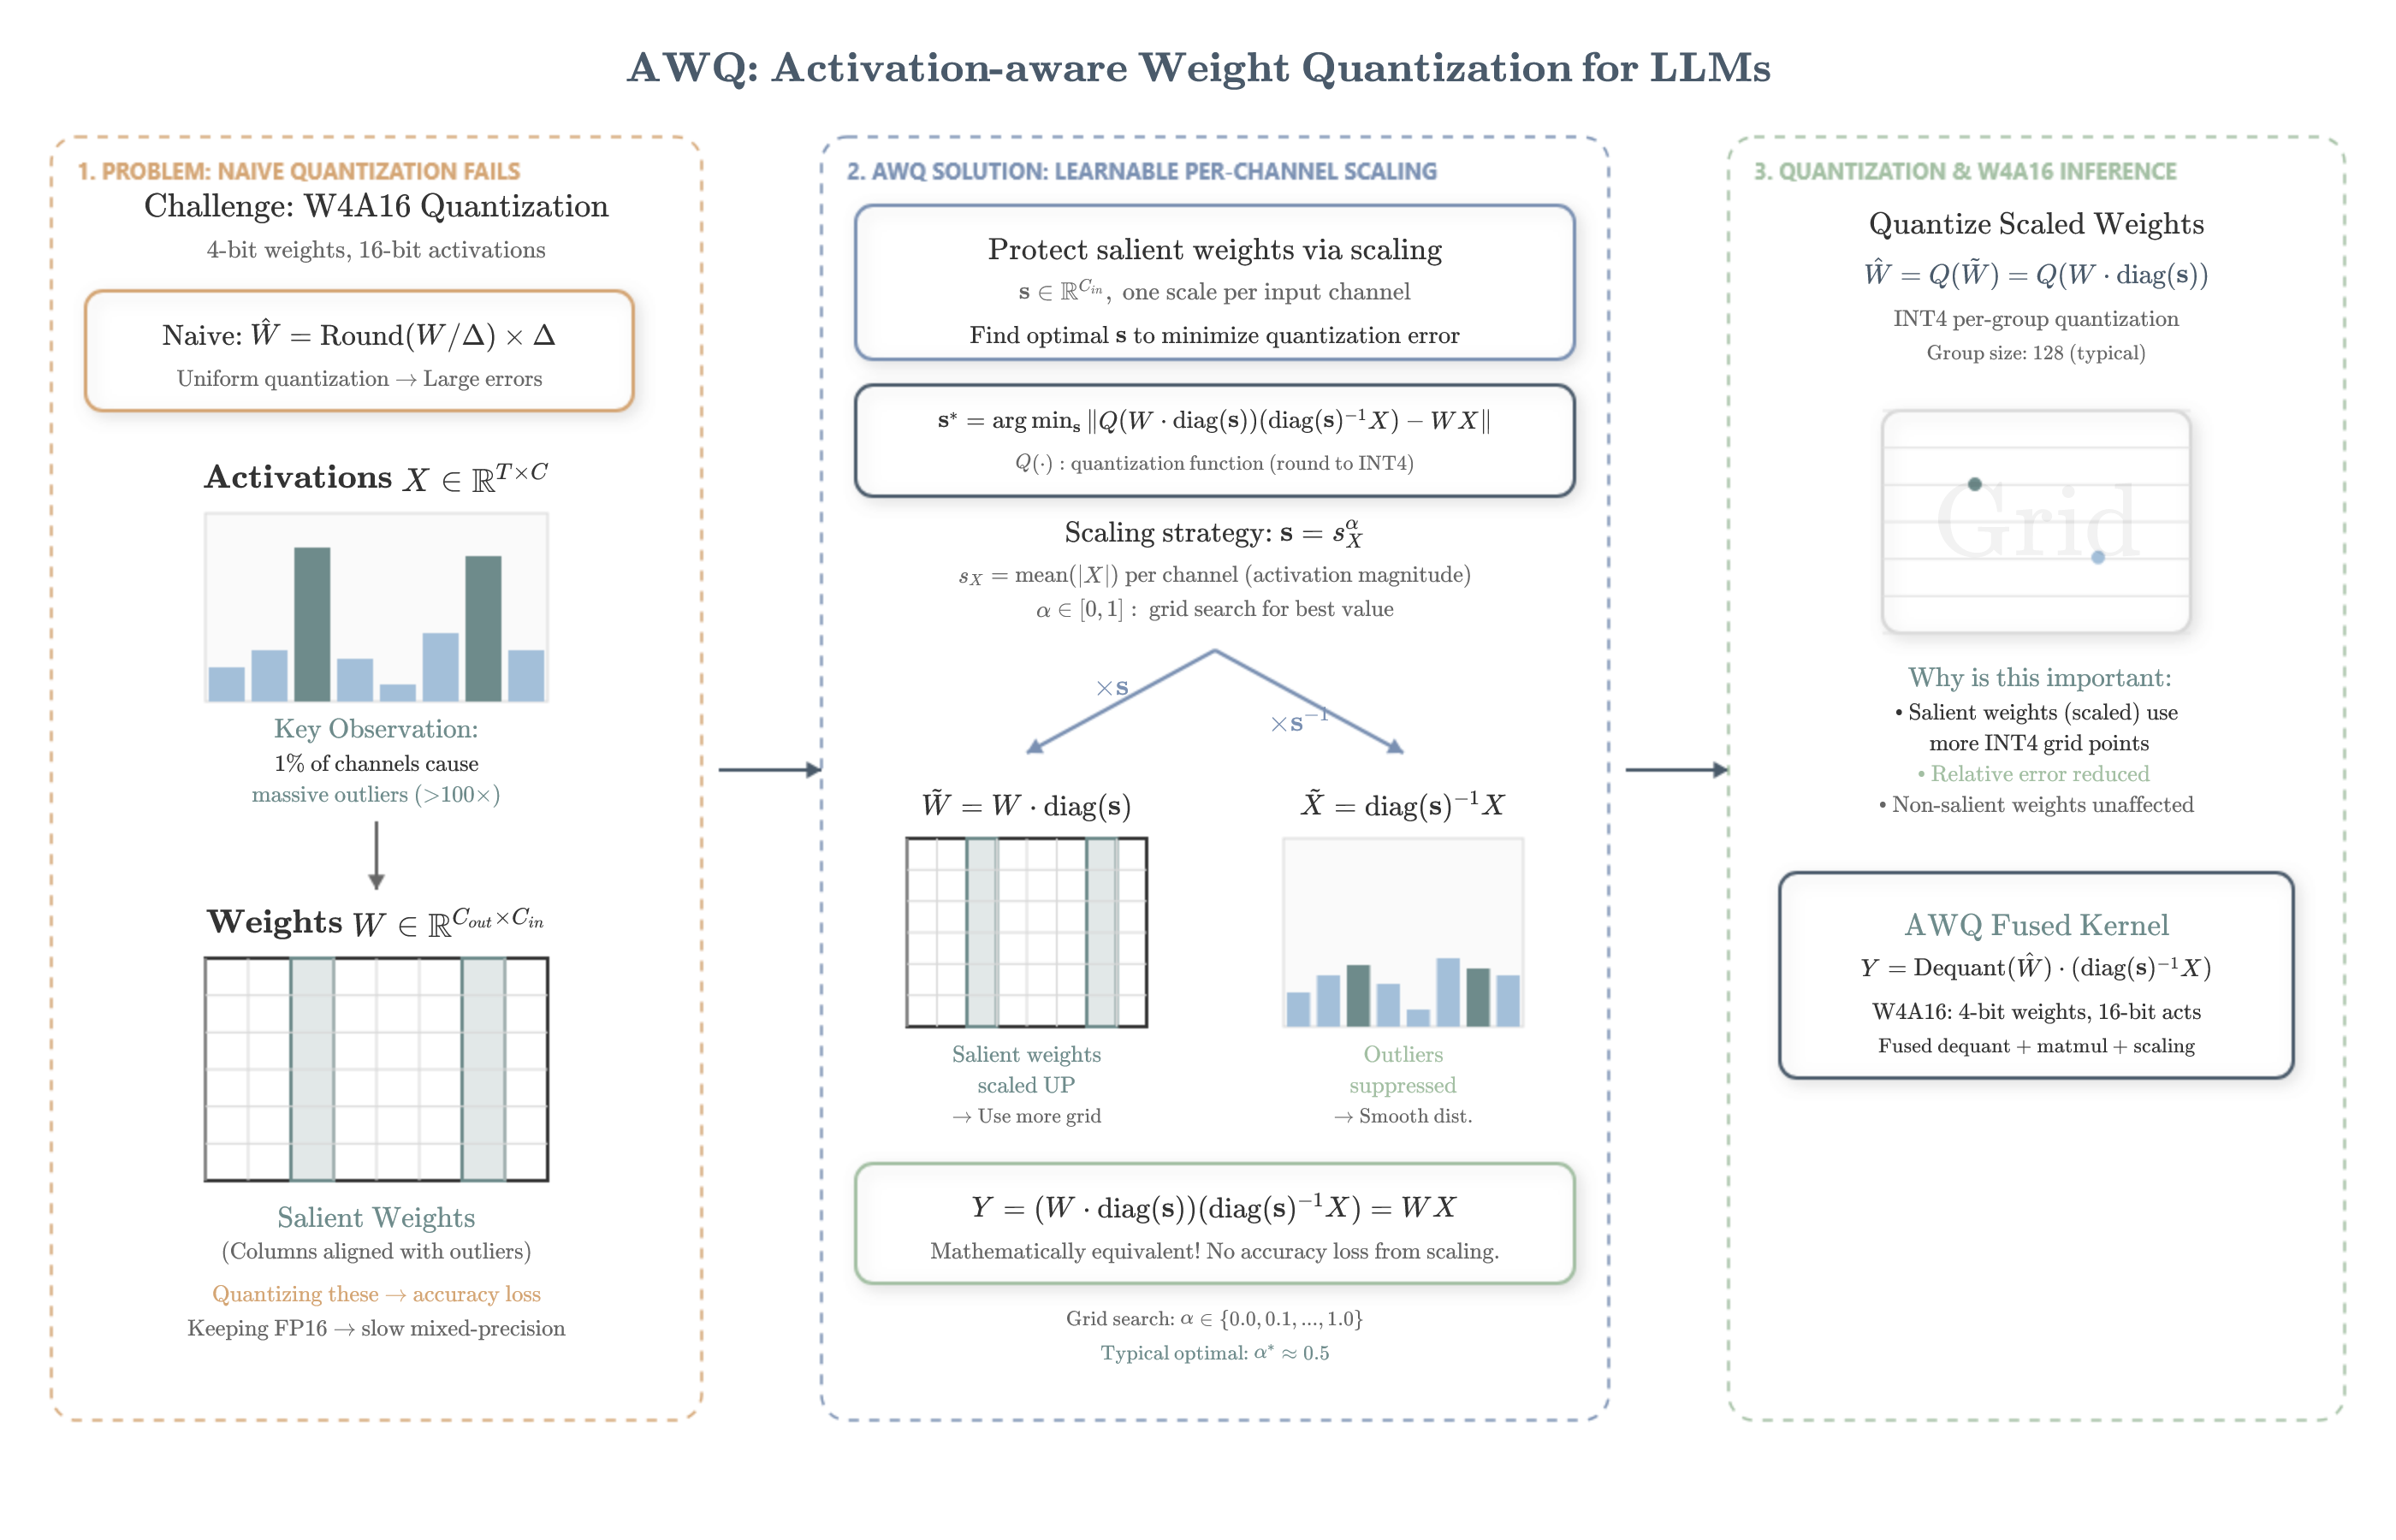
\includegraphics[scale=0.2]{awq_enhanced_diagram.png}%
  }
  \caption{Overview of AWQ. (a) Observation: Weights are not equally important; weights corresponding to channels with large activation magnitudes ("salient channels") are critical for accuracy. (b) Method: Instead of keeping salient weights in FP16 (mixed-precision), AWQ applies channel-wise scaling ($\bm{s}$) to protect them. By scaling up the weight groups and scaling down the activations, the relative quantization error for salient weights is minimized within the 4-bit integer grid.}
  \label{fig:awq}
\end{figure}

\problemp{Problem Statement}
Large Language Models (LLMs) rely heavily on a small fraction (approx 1\%) of "salient weights" that are crucial for performance.
\begin{itemize}
  \item \textbf{The Salience Hypothesis:} Conventional methods assume weight importance is determined by the weight's magnitude ($|w|$). AWQ demonstrates this is false; weight importance is determined by the magnitude of the \textit{activation channels} they consume ($|x|$).
  \item \textbf{The Mixed-Precision Challenge:} Existing solutions tackle outliers by keeping salient weights in FP16 and the rest in INT4. This requires splitting matrices and switching hardware kernels, resulting in severe system overhead and memory access inefficiencies that negate the speedup of quantization.
\end{itemize}

\vspace{1cm}
\problemp{Methodology}
AWQ (Activation-aware Weight Quantization) introduces a method to keep \textit{all} weights in INT4 while preserving the accuracy of the 1\% salient weights. It relies on the mathematical invariance of linear layers to scale transformations.

\subparagraph{1. Protection via Activation-Aware Scaling}
Consider the linear operation $\bm{Y} = \bm{W}\bm{X}$. We can apply a channel-wise scaling factor $\bm{s} \in \mathbb{R}^{C_{in}}$ (diagonal matrix $\bm{S} = \text{diag}(\bm{s})$) to the weights and the inverse to the activations:
\begin{equation}
  \bm{Y} = \bm{W}\bm{X} = \bm{W}\bm{S} \cdot \bm{S}^{-1}\bm{X} = (\bm{W}\bm{S}) \cdot (\bm{X}\bm{S}^{-1})
\end{equation}
The quantization process $Q(\cdot)$ is then applied to the scaled weights. The core insight is that the quantization error for a weight $w$ is fixed by the step size $\Delta$. By scaling up a salient weight group by $s > 1$, the relative error decreases:
\begin{equation}
  \text{Err}(Q(w \cdot s)) \approx \frac{\Delta}{2} \implies \text{Relative Err} \propto \frac{\Delta}{w \cdot s}
\end{equation}
AWQ effectively "dilates" the salient weight channels, allowing them to occupy more quantization levels, while suppressing non-salient channels.

\subparagraph{2. Search Space Optimization}
Finding the optimal scale $\bm{s}$ is an optimization problem. Rather than learning $\bm{s}$ via backpropagation (which risks overfitting the calibration set), AWQ defines a heuristic search space based on activation magnitudes.
Let $\bm{s}_X$ be the average magnitude of activations per channel. The optimal scale is defined as:
\begin{equation}
  \bm{s} = \bm{s}_X^\alpha
\end{equation}
AWQ performs a fast grid search for the hyperparameter $\alpha$ (typically in range $[0, 1]$) to minimize the layer-wise reconstruction error:
\begin{equation}
  \min_{\alpha} \left\| \bm{W}\bm{X} - Q(\bm{W} \cdot \text{diag}(\bm{s}_X^\alpha)) \cdot (\text{diag}(\bm{s}_X^{-\alpha}) \bm{X}) \right\|_2^2
\end{equation}
This search is extremely fast because it only relies on activation statistics from a small calibration set, not full gradient descent.

\subparagraph{3. Efficient Inference Framework}
A key contribution of AWQ is that it does not require runtime floating-point scaling (which would slow down inference).
\begin{itemize}
  \item \textbf{Weight Fusion:} The scaling factor $\bm{S}$ is permanently fused into the weights \textit{before} quantization ($\bm{W}_{int} = Q(\bm{W}\bm{S})$).
  \item \textbf{Activation Scaling:} The inverse scale $\bm{S}^{-1}$ is applied to the activations $\bm{X}$ element-wise. Since element-wise operations are memory-bound but computationally cheap, this has negligible cost compared to the matrix multiplication.
  \item \textbf{Result:} The resulting kernel performs pure INT4 matrix multiplication without the complexity of mixed-precision memory layouts.
\end{itemize}

\problemp{Key Properties and Results}
\begin{itemize}
  \item \textbf{Calibration Robustness:} Unlike GPTQ, which minimizes reconstruction error via Hessian inversion (often overfitting to the calibration set), AWQ's heuristic search preserves generalization. It maintains high performance on instruction-tuned models (e.g., Vicuna) where other methods degrade.
  \item \textbf{Hardware Efficiency:} The paper releases a specialized W4A16 (4-bit weight, 16-bit activation) CUDA kernel. This kernel avoids the need to dequantize weights to global memory, performing dequantization in registers, yielding a $1.45\times$ speedup over GPTQ-triton.
  \item \textbf{Performance:} AWQ achieves perplexity comparable to FP16 on LLaMA-65B and outperforms Round-to-Nearest (RTN) and GPTQ on zero-shot tasks (MMLU, BoolQ), particularly in low-bit regimes or on small calibration sets.
\end{itemize}

\mainp{OWQ}

\begin{figure}[h!]
  \hspace*{-0.5cm}
  \makebox[\textwidth][c]{%
    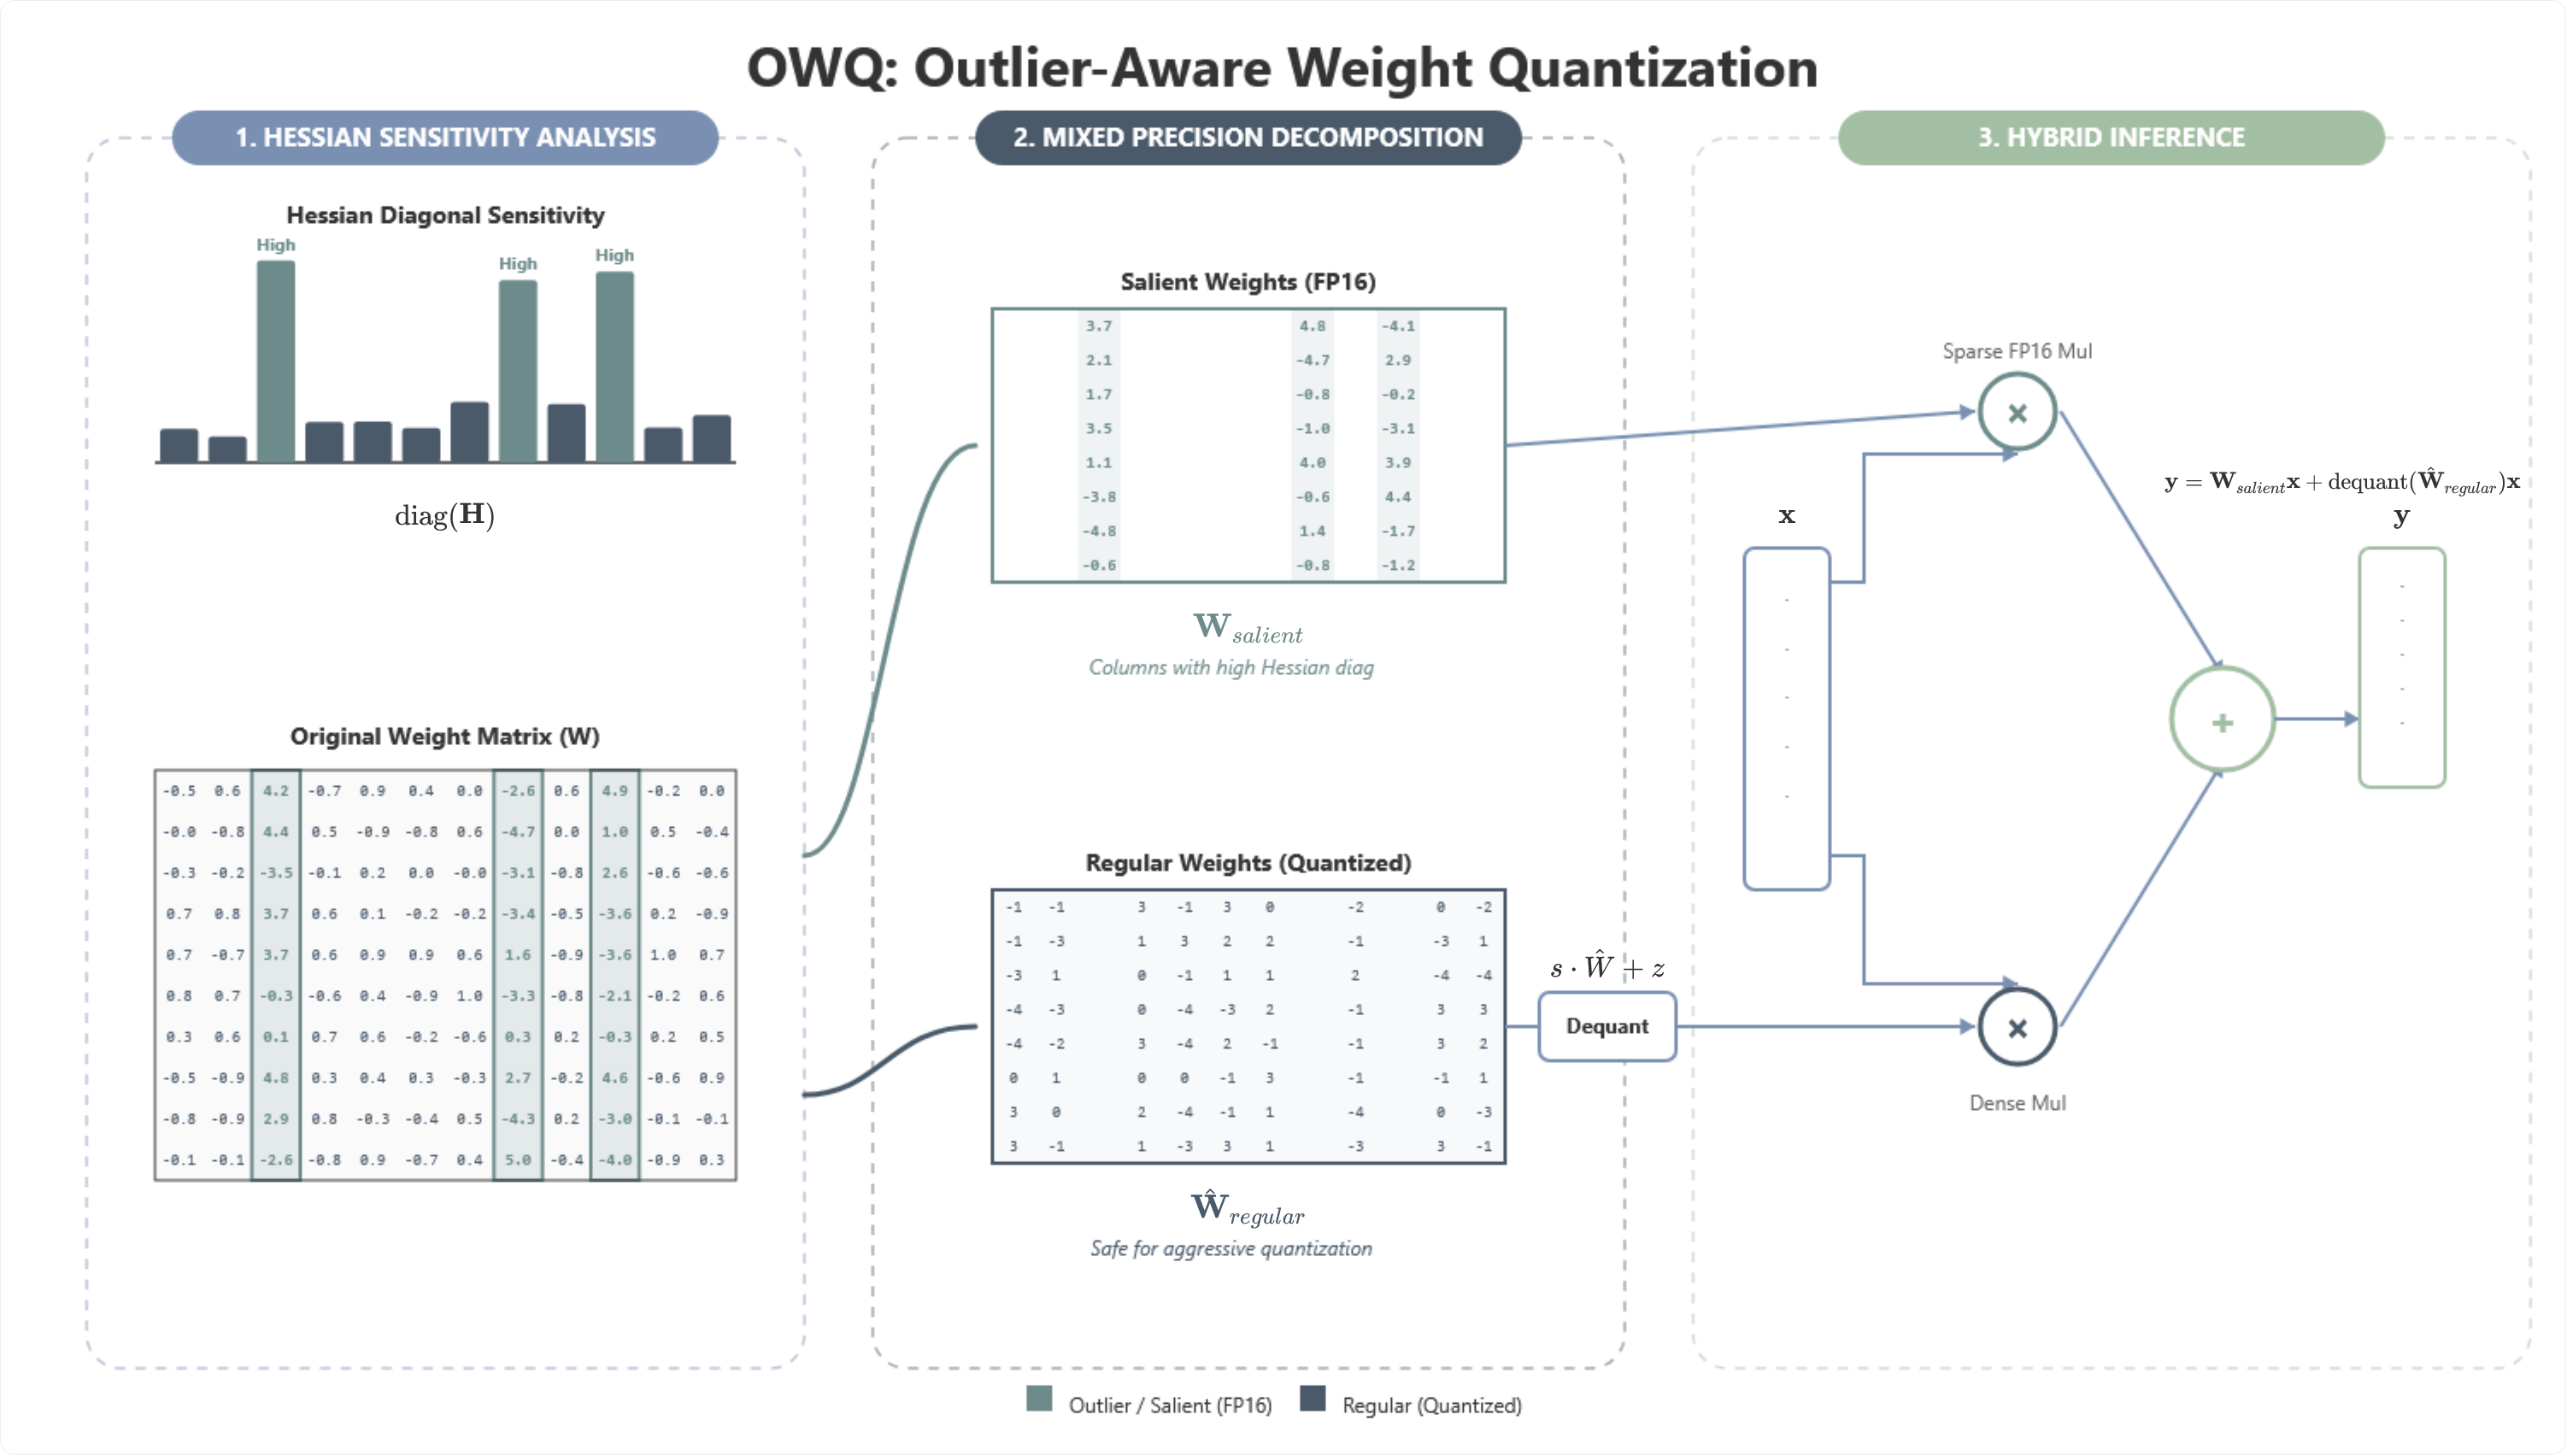
\includegraphics[scale=0.20]{owq-methodology-enhanced.png}%
  }
  \caption{Overview of OWQ (Outlier-Aware Weight Quantization). The method identifies "weak columns" in the weight matrix $\bm{W}$ that correspond to outlier activation channels (high magnitude features). These columns are extremely sensitive to quantization noise. OWQ segregates them into a separate sparse FP16 matrix ($\bm{W}_{\text{weak}}$), while the remaining "strong columns" are quantized to low precision (e.g., 3-bit or 4-bit) using GPTQ. The output is computed as the sum of the quantized path and the high-precision outlier path.}
  \label{fig:owq}
\end{figure}

\problemp{Problem Statement}
Large Language Models exhibit "outlier features", specific activation channels where magnitudes are up to $100\times$ larger than surrounding channels. The quantization error in the output is defined by $\Delta \bm{Y} = \Delta \bm{W} \bm{X}$.
When $\bm{X}$ contains massive outliers, even small quantization errors $\Delta \bm{W}$ in the corresponding weight columns are amplified significantly, dominating the total reconstruction loss. Standard methods like GPTQ treat all weights equally (in terms of bit-width) or rely on activation clipping, which permanently destroys outlier information needed for difficult reasoning tasks.

\vspace{1cm}
\problemp{Methodology}
OWQ proposes a mixed-precision formulation based on sensitivity analysis of the Hessian matrix. Instead of clamping activations or quantizing all weights uniformly, OWQ mathematically selects a subset of weights to preserving in floating point (FP16).

\subparagraph{Theoretical Sensitivity Analysis}
The objective is to minimize the expected output error variance:
\begin{equation}
  \min_{\hat{\bm{W}}} \mathbb{E}\left[ \| (\bm{W} - \hat{\bm{W}})\bm{X} \|_2^2 \right] = \text{Tr}\left( (\bm{W} - \hat{\bm{W}})^\top (\bm{W} - \hat{\bm{W}}) \mathbb{E}[\bm{X}\bm{X}^\top] \right)
\end{equation}
The term $\mathbb{E}[\bm{X}\bm{X}^\top]$ is the empirical Hessian $\bm{H}$. The error contribution of the $i$-th column of $\bm{W}$ is proportional to the $i$-th diagonal element of the Hessian, $\bm{H}_{ii}$, which represents the aggregate power of the $i$-th input feature.
\begin{itemize}
  \item \textbf{Weak Columns:} Columns where $\bm{H}_{ii}$ is large. These weights multiply outlier activations; quantizing them causes high error.
  \item \textbf{Strong Columns:} Columns where $\bm{H}_{ii}$ is small. These can be aggressively quantized with minimal impact.
\end{itemize}

\subparagraph{Algorithm}
OWQ sorts the indices of the weight columns based on their sensitivity $\bm{H}_{ii}$.
\begin{itemize}
  \item \textbf{Step 1: Outlier Selection.} Select the top-$k$ indices with the largest Hessian diagonals to form the set of "weak" columns $S_{\text{weak}}$. The number $k$ is determined by a target memory budget (e.g., equivalent to an average of 3.01 bits per weight).
  \item \textbf{Step 2: Matrix Decomposition.} The weight matrix $\bm{W}$ is decomposed into:
    \begin{equation}
      \bm{W} = \bm{W}_{\text{quant}} + \bm{W}_{\text{weak}}
    \end{equation}
    where $\bm{W}_{\text{weak}}$ contains the FP16 values for columns in $S_{\text{weak}}$ (zeros elsewhere), and $\bm{W}_{\text{quant}}$ contains the remaining columns ready for quantization.
  \item \textbf{Step 3: Quantization.} $\bm{W}_{\text{quant}}$ is quantized using GPTQ (utilizing the inverse Hessian information for rounding) to low bit-widths (e.g., 3-bit).
\end{itemize}

\subparagraph{Inference Kernel}
During inference, the matrix multiplication is split:
\begin{equation}
  \bm{Y} = \text{dequant}(\hat{\bm{W}}_{\text{quant}}) \bm{X} + \bm{W}_{\text{weak}}[\cdot, S_{\text{weak}}] \bm{X}[S_{\text{weak}}, \cdot]
\end{equation}
The second term involves a sparse matrix multiplication (or gather-matmul) focusing only on the high-precision outlier channels.

\problemp{Key Properties and Results}
\begin{itemize}
  \item \textbf{Tremendous Gain at Low Bits:} OWQ significantly outperforms GPTQ and RTN at 3-bit and 4-bit settings. For example, a 3.01-bit OWQ model (3-bit base + 1\% FP16) outperforms a standard 4-bit GPTQ model in many cases.
  \item \textbf{Explanation of Fragility:} It empirically demonstrates that the performance collapse in low-bit LLMs is driven almost entirely by the quantization error in a tiny fraction of weight columns corresponding to activation outliers.
  \item \textbf{No Retraining:} Like GPTQ, OWQ is a Post-Training Quantization (PTQ) method requiring only a small calibration set, avoiding expensive fine-tuning.
  \item \textbf{Pareto Efficiency:} OWQ provides a better trade-off between model size and perplexity than uniform quantization, effectively allocating "bit budget" to where the Hessian indicates it is most needed.
\end{itemize}

 \newpage

\subsubsection{Compensation-Based}
This class updates a subset of weights to offset errors introduced by quantization.
The mechanism rewrites quantization error using curvature information and applies small corrective updates to unquantized weights.

\mainp{GPTQ}

\begin{figure}[h!]
 \hspace*{0cm}
  \makebox[\textwidth][c]{%
    
\includegraphics[scale=0.27]{gptqpng.png}%
  }
  \caption{The GPTQ Algorithm. To avoid the computationally prohibitive row-wise updates of OBQ, GPTQ employs a \textit{Lazy Batch-Update} strategy. It quantizes weights in blocks (e.g., 128 columns). Inside a block, updates are applied eagerly; however, the costly updates to the global Hessian/remaining weights are delayed until the entire block is processed, reducing memory access overhead significantly.}
  \label{fig:gptq}
\end{figure}
\problemp{Problem Statement}
Generative Pre-trained Transformers (GPT) with billions of parameters (e.g., OPT-175B, BLOOM) require immense GPU memory for inference. While \textit{Optimal Brain Quantization (OBQ)} provides high-accuracy quantization by utilizing second-order information (the Hessian), its computational complexity is $O(d_{\text{row}}\cdot d_{\text{col}}^{3})$, which makes it infeasible for very large layers. For a 175B model, OBQ would take months to execute. Standard Round-to-Nearest (RTN) is fast but destroys accuracy. The challenge is to scale second-order quantization to billion-parameter models with a runtime comparable to a standard forward pass. 

\vspace{1cm}
\problemp{Methodology}
GPTQ is a one-shot weight quantization method based on approximate second-order information. It solves the layer-wise reconstruction problem:
\begin{equation}
    \hat{\bm{W}} \;=\; \arg\min_{\tilde{\bm{W}}} \, \| \bm{W}\bm{X} - \tilde{\bm{W}}\bm{X} \|_{F}^{2},
    \label{eq:layer-recons}
\end{equation}
where $\|\cdot\|_{F}$ denotes the Frobenius norm, $\bm{W}\in\mathbb{R}^{d_{\text{row}}\times d_{\text{col}}}$ is the full-precision weight matrix and $\bm{X}\in\mathbb{R}^{d_{\text{col}}\times m}$ contains $m$ calibration inputs.

Using trace identities,
\begin{equation}
    \| \bm{W}\bm{X} - \tilde{\bm{W}}\bm{X} \|_{F}^{2}
    \;=\;
    \operatorname{Tr}\!\big( (\bm{W}-\tilde{\bm{W}})\,\bm{X}\bm{X}^\top(\bm{W}-\tilde{\bm{W}})^\top \big).
    \label{eq:trace-form}
\end{equation}
If we focus on a single output row $\bm{w}\in\mathbb{R}^{d_{\text{col}}}$ of $\bm{W}$ (as OBQ does), the per-row scalar objective becomes
\[
    \ell(\tilde{\bm{w}})
    \;=\;
    \| \bm{w}\bm{X} - \tilde{\bm{w}}\bm{X} \|_{2}^{2}
    \;=\;
    (\bm{w}-\tilde{\bm{w}})^\top \!\big(\bm{X}\bm{X}^\top\big)\,(\bm{w}-\tilde{\bm{w}}).
\]
Thus the Hessian w.r.t.\ a single row $\bm{w}$ is
\begin{equation}
    \bm{H} \;=\; 2\,\bm{X}\bm{X}^\top,
    \label{eq:hessian}
\end{equation}
and the quadratic form can be written as
\begin{equation}
    \ell(\tilde{\bm{w}}) \;=\; \tfrac{1}{2}\,(\bm{w}-\tilde{\bm{w}})^\top \bm{H} (\bm{w}-\tilde{\bm{w}}).
    \label{eq:half-hessian}
\end{equation}
(That 1/2 factor is important: if $\ell(\cdot)=(\bm{w}-\tilde{\bm{w}})^\top\!A(\bm{w}-\tilde{\bm{w}})$ then the Hessian is $2A$.)

GPTQ builds on OBQ’s second-order approximation but adds three practical algorithmic innovations that make it scalable.

\subparagraph{1. Arbitrary-order insight}
OBQ selects the next weight greedily to minimize the instantaneous increase in loss and updates the inverse Hessian repeatedly; this gives a per-weight cubic cost across columns. GPTQ observes that, for large layers, fixing a simple order (processing columns/weights in a fixed, e.g., row-by-row / column-major order) yields negligible accuracy loss, which avoids the expensive sorting/selection steps and allows much more structure in the updates.

\subparagraph{2. Cholesky reformulation}
OBQ needs rows of the inverse Hessian $\bm{H}^{-1}$ to compute how the quantization of one weight affects the others. The scalar one-weight update (OBQ notation) for quantizing weight index $q$ (with remaining set $F$) is:
\begin{align}
    w_q &= \arg\min_{w_q} \frac{(\operatorname{quant}(w_q)-w_q)^2}{\big[\bm{H}_F^{-1}\big]_{qq}}, \\
    \delta_F &= - \frac{w_q - \operatorname{quant}(w_q)}{\big[\bm{H}_F^{-1}\big]_{qq}} \ (\bm{H}_F^{-1})_{:,q},
    \label{eq:obq-update}
\end{align}
which matches the OBQ formulas. Computing and repeatedly updating $\bm{H}^{-1}$ directly can be numerically unstable and costly. GPTQ instead precomputes a Cholesky factorization of the (damped) inverse Hessian,
\begin{equation}
    \bm{H}^{-1} \;=\; \bm{L}\bm{L}^\top,
\end{equation}
with $\bm{L}$ lower-triangular. Using $\bm{L}$ lets one obtain the required columns/rows of $\bm{H}^{-1}$ stably (and with better numerical conditioning), and to propagate quantization errors via the triangular factors. The paper also explains the small technical detail that Cholesky-based row extraction differs from the one-step Gaussian-elimination formula by a diagonal square-root scaling; GPTQ leverages optimized Cholesky kernels combined with mild dampening to avoid indefiniteness.

\subparagraph{3. Lazy batch-updates}
Updating the entire (possibly huge) weight matrix for every single quantized scalar is memory-bandwidth bound. GPTQ processes columns in blocks of size $B$ (e.g., $B=128$). For a block of indices $Q$ the multi-weight versions of the OBQ updates are:
\begin{align}
    \delta_F &= - ( \bm{w}_Q - \operatorname{quant}(\bm{w}_Q) ) \cdot \big( [\bm{H}_F^{-1}]_{QQ} \big)^{-1} \, (\bm{H}_F^{-1})_{:,Q}, \label{eq:multi-delta} \\
    \bm{H}^{-1}_{-Q} &= \bm{H}^{-1} - \bm{H}^{-1}_{:,Q} \, \big( [\bm{H}^{-1}]_{QQ} \big)^{-1} \, \bm{H}^{-1}_{Q,:}. \label{eq:schur}
\end{align}
During the block (intra-block) step GPTQ only updates columns within the block using local Cholesky information; once the block is complete it performs a single global matrix update of the remaining columns:
\begin{equation}
    \bm{W}_{:,(i+B):} \;\leftarrow\; \bm{W}_{:,(i+B):} - \bm{E}\,\bm{H}^{-1}_{\,i:(i+B),\,(i+B):},
    \label{eq:block-update}
\end{equation}
where $\bm{E}$ aggregates the per-column quantization errors inside the block. This raises arithmetic intensity and enables efficient GPU utilization. 

\problemp{Key Properties and Results}
\begin{itemize}
    \item \textbf{Complexity:} GPTQ reduces the runtime of OBQ by several orders of magnitude by (i) sharing the same column-order across rows, (ii) performing block (lazy) updates, and (iii) using Cholesky-based precomputation. Concretely, the runtime is reduced from $O(d_{\text{row}}\cdot d_{\text{col}}^{3})$ (OBQ) to $O\!\big(\max\{d_{\text{row}}\cdot d_{\text{col}}^{2},\, d_{\text{col}}^{3}\}\big)$ in practice. 
    \item \textbf{Accuracy and scale:} GPTQ can quantize OPT-175B (and similar models) to 3–4 bits with negligible perplexity degradation and can quantize a 175B model in ~4 GPU hours (single A100) using 128 calibration samples, per the paper’s experiments. 
    \item \textbf{Bit-width flexibility and no retraining:} Supports 4/3/2-bit regimes (2-bit typically requires smaller blocks/grouping) and is pure post-training quantization requiring only small calibration data.
\end{itemize}

\newpage
\mainp{VPTQ}

\begin{figure}[h!]
 \hspace*{1cm}
  \makebox[\textwidth][c]{%
    \includegraphics[scale=0.4]{vptq_architecture.png}%
  }
  \caption{VPTQ Methodology. Weights are reshaped into vectors $\bm{v}$. A Second-Order optimizer iteratively solves for the optimal codebook centroids $\mathcal{C}$ and indices $\bm{I}$ by minimizing the Hessian-weighted error. Unlike scalar quantization, VPTQ captures local correlations within the vector. During inference, dequantization is reduced to a zero-overhead Lookup Table (LUT) operation, bypassing complex bit-shifting logic.}
  \label{fig:vptq}
\end{figure} 

\problemp{Problem Statement}
Scalar quantization (SQ) methods (e.g., GPTQ, AWQ) hit a fundamental "compression wall" below 3 bits. At 2 bits or 1 bit, the limited discrete values of scalar rounding cannot preserve the model's spectral properties, leading to collapse. Furthermore, standard Vector Quantization (VQ) is historically intractable for LLMs due to the $O(K \cdot N)$ search complexity and the lack of second-order (Hessian) guidance, resulting in poor alignment with the task loss landscape.

\vspace{1cm}
\problemp{Methodology}
VPTQ (Vector Post-Training Quantization) reformulates LLM compression as a **Second-Order Vector Quantization** problem. It combines the granularity of VQ with the Hessian-based error correction of Optimal Brain Surgeon. The method minimizes the following proxy objective for a weight matrix $\bm{W}$ reshaped into a collection of vectors $\mathcal{V} = \{ \bm{v}_1, \dots, \bm{v}_n \}$:

\begin{equation}
    \min_{\mathcal{C}, \mathcal{I}} \sum_{j=1}^n (\bm{v}_j - \bm{c}_{I_j})^\top \bm{H}_{\bm{v}} (\bm{v}_j - \bm{c}_{I_j})
\end{equation}
where $\mathcal{C} = \{ \bm{c}_1, \dots, \bm{c}_K \}$ is the codebook, $\mathcal{I}$ are the indices, and $\bm{H}_{\bm{v}}$ is the Hessian block corresponding to the vector dimension.

\subparagraph{1. Vector-wise Second-Order Optimization}
Unlike scalar methods that treat weights independently or row-wise, VPTQ quantizes vectors of dimension $d$ (e.g., $1 \times 8$). The algorithm employs an iterative coordinate descent strategy:
\begin{itemize}
    \item \textbf{Centroid Initialization:} A Hessian-weighted K-Means++ algorithm initializes the codebook $\mathcal{C}$ to align with high-curvature directions of the loss landscape.
    \item \textbf{Index Assignment:} For a vector $\bm{v}_j$, the optimal index $k^*$ is selected by minimizing the quadratic distance:
    \begin{equation}
        k^* = \operatorname*{argmin}_{k} \|\bm{L}^\top (\bm{v}_j - \bm{c}_k)\|_2^2
    \end{equation}
    where $\bm{H} \approx \bm{L}\bm{L}^\top$. This metric accounts for the sensitivity of different weights within the vector.
\end{itemize}

\subparagraph{2. Hessian-Guided Error Propagation (Vector-OBS)}
To handle the inter-vector dependencies, VPTQ extends the GPTQ error compensation mechanism to the vector domain. After quantizing vector $\bm{v}_j$ to $\hat{\bm{v}}_j$, the quantization error $\bm{\delta}_j = \bm{v}_j - \hat{\bm{v}}_j$ is propagated to the remaining unquantized vectors $\{\bm{v}_{j+1}, \dots \}$ using the inverse Hessian $\bm{H}^{-1}$:
\begin{equation}
    \bm{W}_{:, k} \leftarrow \bm{W}_{:, k} - \frac{[\bm{H}^{-1}]_{kj}}{[\bm{H}^{-1}]_{jj}} \bm{\delta}_j
\end{equation}
This ensures that future vector quantization steps compensate for the errors introduced by previous steps, preserving the global function output.

\subparagraph{3. Residual Quantization (IVQ)}
For extreme compression (e.g., < 2 bits equivalent), VPTQ employs Iterative Vector Quantization (IVQ). After the primary quantization, a secondary codebook is trained on the residuals:
\begin{equation}
    \bm{r}_j = \bm{v}_j - \bm{c}^{(1)}_{I_j}, \quad \bm{r}_j \approx \bm{c}^{(2)}_{K_j}
\end{equation}
This "residual codebook" exponentially reduces the quantization error variance without significantly increasing the storage cost, as the codebooks are shared across the layer.

\problemp{Key Properties and Results}
\begin{itemize}
    \item \textbf{Breakthrough at 1-2 Bits:} VPTQ is one of the few methods to achieve coherent generation on Llama-3-70B at $\sim$2 bits, significantly outperforming QuIP\# and AQLM in perplexity (e.g., Llama-2-7B at 2-bit achieves 6.64 PPL vs 11.23 for GPTQ).
    \item \textbf{Inference Throughput (The LUT Advantage):} Unlike scalar bit-packing which requires bitwise logic and shifting during decoding, VPTQ dequantization is a pure memory-bound Lookup Table (LUT) operation. This results in a $1.6\times - 1.8\times$ inference speedup over SOTA kernels.
    \item \textbf{Domain Parallelism:} By treating weights as vectors, the codebook size $K$ allows for fractional bit-widths (e.g., $\frac{\log_2 K}{dim}$ bits per weight), offering a continuous trade-off curve between model size and accuracy.
\end{itemize}



\subsubsection{Optimization-Based}
This class searches for quantization parameters that minimize the mismatch between the full-precision model and the quantized one.
The representative approach, \textbf{OmniQuant}, performs block-wise learning where full-precision outputs guide the updates of scaling parameters, reducing the deviation
$\|F(W, X) - F(Q_w(W; \Theta), X)\|$.
Further developments include \textbf{CBQ}, \textbf{LRQuant} (using nonlinear coherence losses), and \textbf{AffineQuant}, which introduces learned affine transformations to refine quantization behavior.



\mainp{OmniQuant}

\begin{figure}[h!]
 \hspace*{1cm}
  \makebox[\textwidth][c]{%
    \includegraphics[scale=0.4]{omniquant_pipeline.png}%
  }
  \caption{OmniQuant Methodology. Unlike PTQ methods that rely on hand-crafted heuristics (e.g., SmoothQuant's migration strength $\alpha$) or greedy search (AWQ), OmniQuant freezes the original weights and learns the quantization parameters via gradient descent. It optimizes two components simultaneously: Learnable Weight Clipping (LWC) for weight quantization and Learnable Equivalent Transformation (LET) for activation outlier mitigation.}
  \label{fig:omniquant}
\end{figure}

\problemp{Problem Statement}
Post-Training Quantization (PTQ) usually relies on heuristic rules to determine quantization parameters (e.g., min-max clipping or analyzing activation magnitude statistics). Methods like SmoothQuant utilize a manually tuned hyperparameter to migrate quantization difficulty from activations to weights. Conversely, Quantization-Aware Training (QAT) yields high accuracy but is computationally prohibitive for LLMs. OmniQuant bridges this gap by introducing a **differentiable calibration** scheme that is fast like PTQ but powerful like QAT.

\vspace{1cm}
\problemp{Methodology}
OmniQuant retains the original full-precision weights $\bm{W}$ but learns the optimal quantization configuration by minimizing the layer-wise reconstruction loss $\mathcal{L} = \|\bm{Y} - \hat{\bm{Y}}\|_F^2$ using stochastic gradient descent. The method decomposes the quantization difficulty into two learnable operators:

\subparagraph{1. Learnable Weight Clipping (LWC)}
Standard methods clamp weights based on static statistics (e.g., absolute max). OmniQuant treats the clipping thresholds as learnable parameters. For a weight matrix $\bm{W}$, the quantization range $[\gamma_l, \gamma_u]$ is optimized:
\begin{equation}
    \hat{\bm{W}} = \text{Clamp}\left(\left\lfloor \frac{\bm{W} - \gamma_l}{s_w} \right\rceil \cdot s_w + \gamma_l, \gamma_l, \gamma_u\right), \quad s_w = \frac{\gamma_u - \gamma_l}{2^b - 1}
\end{equation}
Here, $\gamma_l$ and $\gamma_u$ are optimized via backpropagation. This allows the model to dynamically choose whether to preserve the median distribution or accommodate outlier weights based on their actual impact on the output error, effectively outperforming the heuristic grid-search used in AWQ.

\subparagraph{2. Learnable Equivalent Transformation (LET)}
To handle activation outliers (essential for W4A4 quantization), OmniQuant exploits the mathematical equivalence of linear layers. It learns a channel-wise scaling vector $\bm{s}$ that shifts the outlier challenge from activations $\bm{X}$ to weights $\bm{W}$:
\begin{equation}
    \bm{Y} = \bm{X}\bm{W}^\top = (\bm{X} \cdot \text{diag}(\bm{s})) (\text{diag}(\bm{s})^{-1} \bm{W}^\top)
\end{equation}
Unlike SmoothQuant, which calculates $\bm{s}$ using a fixed formula $s_j = \max(|X_j|)^\alpha / \max(|W_j|)^{1-\alpha}$, OmniQuant treats $\bm{s}$ as a free parameter optimized alongside the LWC bounds. This learns the optimal "migration" of outliers for every specific channel, rather than relying on a global assumption.

\subparagraph{3. Block-wise Optimization}
The optimization is performed block-by-block. For each Transformer block, the original weights are frozen. The parameters $\Theta = \{ \gamma_l, \gamma_u, \bm{s} \}$ are updated using the gradients derived from the reconstruction loss:
\begin{equation}
    \Theta^* = \operatorname*{argmin}_{\Theta} \mathbb{E}_{\bm{X}} \left[ \| \text{Block}(\bm{X}) - \text{QuantBlock}(\bm{X}; \Theta) \|_F^2 \right]
\end{equation}
To handle the non-differentiable rounding operation $\lfloor \cdot \rceil$, OmniQuant employs the Straight-Through Estimator (STE), allowing gradients to propagate to the clipping bounds and scaling factors.

\problemp{Key Properties and Results}
\begin{itemize}
    \item \textbf{Heuristic-Free:} Eliminates the need for manual hyperparameter tuning (like the $\alpha$ in SmoothQuant) or expensive search spaces (like AWQ), replacing them with standard gradient descent.
    \item \textbf{W4A4 Capability:} Enables effective 4-bit weight and 4-bit activation quantization on Llama-2 models, a regime where standard PTQ methods typically fail due to activation outliers.
    \item \textbf{No Inference Overhead:} The learned transformations (LET) are fused into the weights and activation quantization parameters offline. The inference graph remains a standard quantized matrix multiplication without additional runtime operators.
    \item \textbf{Versatility:} The method works seamlessly for both Weight-Only (W4A16) and Weight-Activation (W4A4) settings, consistently outperforming GPTQ and SmoothQuant in perplexity metrics (e.g., LLaMA-30B W4A16 perplexity 7.21 vs 7.64 for GPTQ).
\end{itemize}


\mainp{LRQuant}

\begin{figure}[h!]
 \hspace*{0cm}
  \makebox[\textwidth][c]{%
    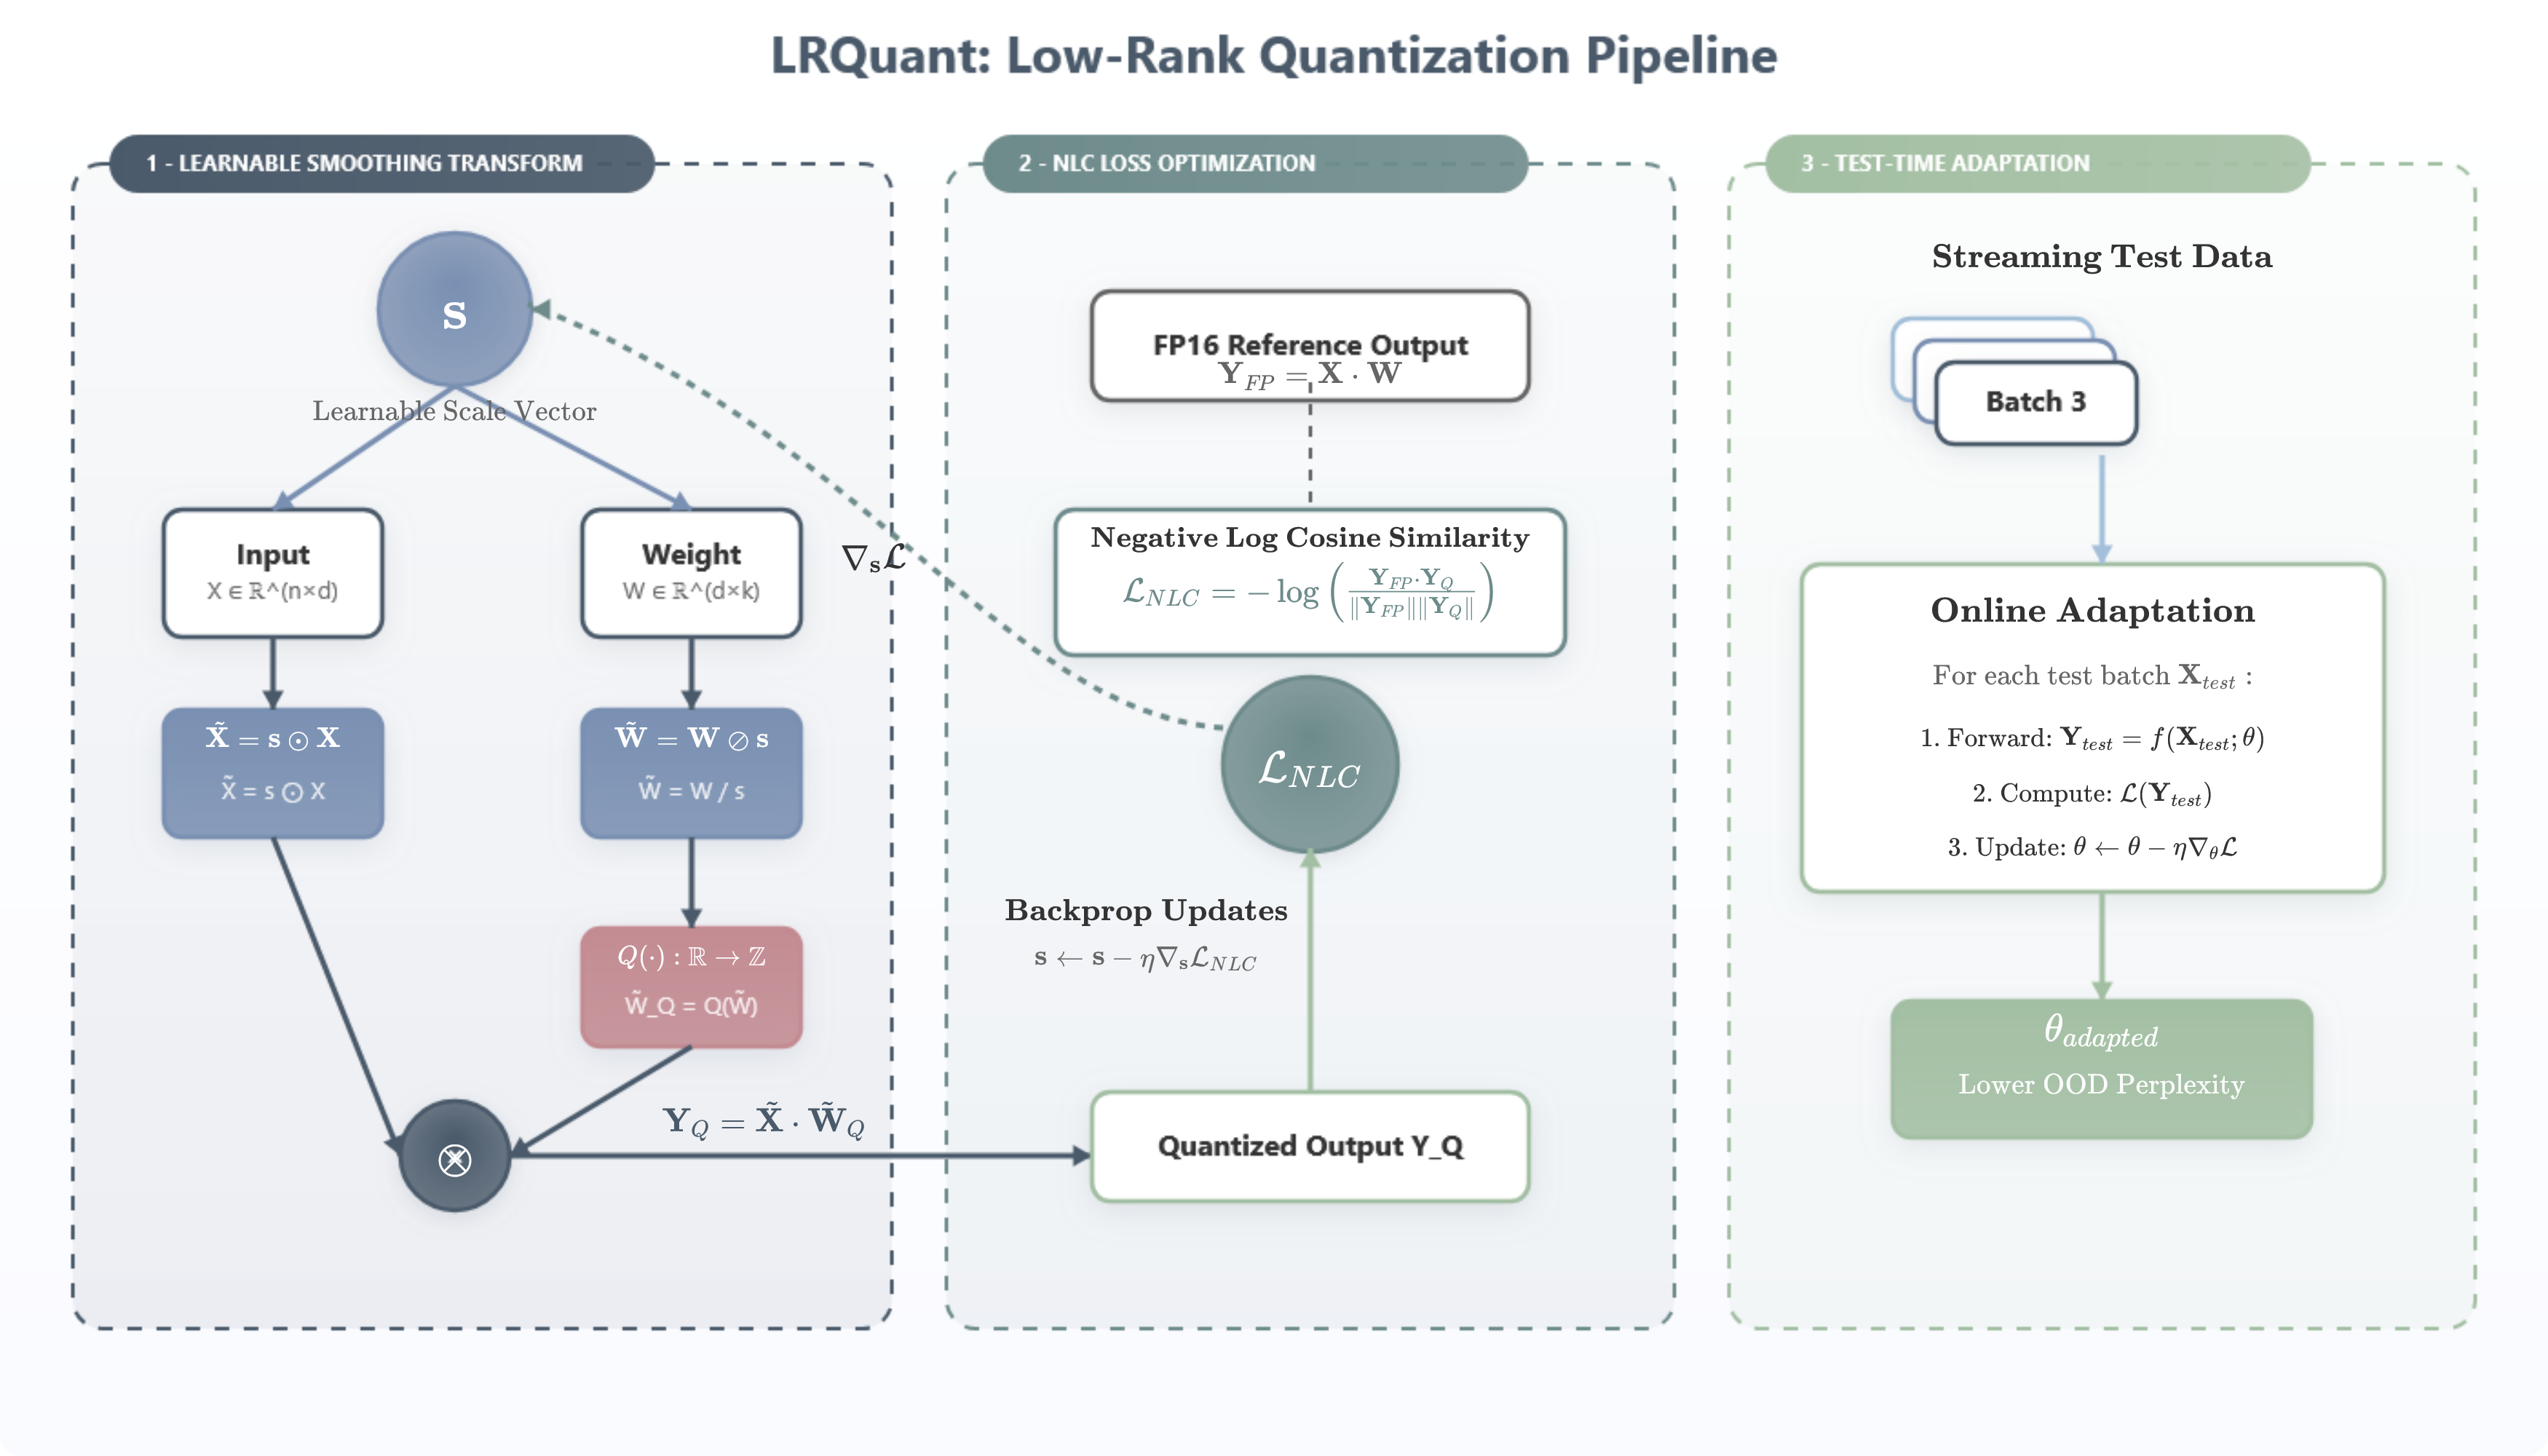
\includegraphics[scale=0.16]{LRQuant_Enhanced_Diagram.png}%
  }
  \caption{LRQuant Methodology. (a) \textbf{Learnable Smoothing}: Instead of using heuristic hyperparameters (like SmoothQuant's $\alpha$), LRQuant treats the smoothing scales $\mathbf{s}$ as learnable parameters, optimized via gradient descent. (b) \textbf{NLC Loss}: A novel Negative Log-Cosine loss replaces MSE to better align the semantic directions of the quantized output. (c) \textbf{Test-Time Adaptation (TTA)}: During inference, the quantization parameters are dynamically updated on the incoming test stream to combat distribution shifts.}
  \label{fig:lrquant}
\end{figure}

\problemp{Problem Statement}
Existing Post-Training Quantization (PTQ) methods like SmoothQuant rely on "smoothing", transferring the outlier difficulty from activations to weights using a mathematically equivalent transformation. However, these methods typically use \textit{hand-crafted} hyperparameters (e.g., a static migration strength $\alpha$) which are suboptimal for diverse layers. Furthermore, they suffer from poor generalization on unseen datasets (distribution shift) and rely on the Mean Squared Error (MSE) metric, which does not necessarily correlate with the model's semantic generation quality.

\vspace{1cm}
\problemp{Methodology}
LRQuant (Learnable and Robust Quantization) proposes an end-to-end differentiable framework that moves beyond static heuristics. It introduces three key innovations to ensure high-fidelity 4-bit and 8-bit quantization:

\subparagraph{1. Learnable Smoothing Paradigm}
Instead of calculating smoothing scales $\mathbf{s}$ based on fixed activation statistics (max/min), LRQuant defines $\mathbf{s}$ as a learnable parameter. The transformation for weights $\bm{W}$ and input $\bm{X}$ is:
\begin{equation}
    \hat{\bm{W}} = \bm{W} \cdot \text{diag}(\mathbf{s})^{-1}, \quad \hat{\bm{X}} = \text{diag}(\mathbf{s}) \cdot \bm{X}
\end{equation}
These parameters are initialized using a "Logarithmic Activation Equivalent" strategy to ensure stable starting points, then fine-tuned via gradient descent to minimize the reconstruction error of the layer output.

\subparagraph{2. NLC Loss (Negative Log-Cosine)}
The authors identify that MSE focuses on element-wise magnitude errors, which can be misleading for LLM generation where token semantics (direction) matter more than absolute magnitude. LRQuant replaces MSE with the Negative Log-Cosine similarity loss:
\begin{equation}
    \mathcal{L}_{\text{NLC}} = - \log \left( \frac{\bm{Y}_{\text{FP}} \cdot \bm{Y}_{\text{Q}}}{\| \bm{Y}_{\text{FP}} \|_2 \| \bm{Y}_{\text{Q}} \|_2} \right)
\end{equation}
Minimizing $\mathcal{L}_{\text{NLC}}$ maximizes the cosine similarity between the full-precision output $\bm{Y}_{\text{FP}}$ and quantized output $\bm{Y}_{\text{Q}}$, ensuring the token representation vectors point in the correct semantic direction.

\subparagraph{3. Test-Time Adaptation (TTA)}
To handle distribution shifts (e.g., moving from calibration data to real-world prompts), LRQuant introduces a lightweight adaptation phase during inference. For a batch of test inputs, the method performs a few rapid gradient steps on the quantization parameters (scales and bias) to minimize the discrepancy on the *current* data stream.
\begin{equation}
    \theta_{\text{test}} \leftarrow \theta_{\text{test}} - \eta \nabla_{\theta} \mathcal{L}(\bm{X}_{\text{test}})
\end{equation}
This allows the quantizer to "adapt" to the specific activation outliers present in the user's prompt, a feature unique to this framework.

\problemp{Key Properties and Results}
\begin{itemize}
    \item \textbf{Heuristic-Free:} Eliminates the need for manual tuning of the smoothing factor $\alpha$, finding the mathematically optimal distribution of outliers between weights and activations.
    \item \textbf{Generalization:} Significantly outperforms baselines (like SmoothQuant and AWQ) on out-of-distribution datasets due to the robust NLC loss landscape.
    \item \textbf{Efficiency:} The TTA overhead is negligible compared to the decoding time but provides a consistent perplexity recovery on difficult benchmarks.
    \item \textbf{Performance:} Achieves near FP16 performance on LLaMA and OPT families at W4A8 (4-bit weights, 8-bit activations), effectively solving the "outlier channel" problem without complex mixed-precision arithmetic.
\end{itemize}


\newpage
\bibliographystyle{plainnat}
\bibliography{ref}

\end{document}
